% PREAMBLE
\documentclass[12pt]{article}
\usepackage[top=1.2in, bottom=1in, left=1in, right=1in]{geometry}
\usepackage{setspace}
\usepackage{amsfonts}
\usepackage{amsmath}
\usepackage{amssymb}
\usepackage{graphicx}
\usepackage{xcolor}
\usepackage{color}
\usepackage{listings}
\usepackage{parskip}
\usepackage{enumerate}
\usepackage{relsize}
\usepackage{hyperref}
\usepackage{tikz}
\usepackage{caption}
\usepackage{subcaption}


\usepackage{float}
\restylefloat{table}
\restylefloat{figure}

% HEADERS AND FOOTERS
\usepackage{fancyhdr}
\usepackage{lastpage}
%\pagestyle{fancy}
\fancyhead{}
\fancyfoot{}
%\lhead{CS 4700 HW3}

\newenvironment{graphic}[1]{\begin{center}
        \includegraphics[width=0.6\textwidth]{#1}}
        {\end{center}}
        
% CODE STYLE
\definecolor{dkgreen}{rgb}{0,0.6,0}
\definecolor{gray}{rgb}{0.5,0.5,0.5}
\definecolor{mauve}{rgb}{0.58,0,0.82}
\lstset{
  language=python,                % the language of the code
  basicstyle=\ttfamily,           % the size of the fonts that are used for the code
  numbers=left,                   % where to put the line-numbers
  numberstyle=\tiny\color{gray},  % the style that is used for the line-numbers
  stepnumber=1,                   % the step between two line-numbers. If it's 1, each line will be numbered
  numbersep=8pt,                  % how far the line-numbers are from the code
  backgroundcolor=\color{white},      % choose the background color. You must add \usepackage{color}
  showspaces=false,               % show spaces adding particular underscores
  showstringspaces=false,         % underline spaces within strings
  showtabs=false,                 % show tabs within strings adding particular underscores
  rulecolor=\color{black},        % if not set, the frame-color may be changed on line-breaks within not-black text (e.g. comments (green here))
  tabsize=2,                      % sets default tabsize to 2 spaces
  captionpos=b,                   % sets the caption-position to bottom
  breaklines=true,                % sets automatic line breaking
  breakatwhitespace=false,        % sets if automatic breaks should only happen at whitespace
  keywordstyle=\color{blue},          % keyword style
  commentstyle=\color{dkgreen},       % comment style
  stringstyle=\color{mauve},         % string literal style
}

% DOCUMENT
\begin{document}

\begin{center}
\Large{\textbf{Handwritten Digit Recognition}} \\ Chris Heelan (cjh276) \\ Bok Young Kim (bk294)
\end{center}

\section*{Introduction}
In this project, we attempt to recognize handwritten digit characters using a variety of machine learning techniques. Handwritten character recognition is a challenging problem because each person has a slightly different way of writing characters, and there is also the potential for smudges or misprints to cause noise in the data. However, character recognition is very useful, as it can be applied to prescription fulfillments, automated check processing, and postal mail parsing. This project experiments with two different methods of feature extraction - grayscale images and black and white images, along with three different learning algorithms - Support Vector Machines (SVMs), decision trees, and random forests. Using these algorithms, we obtained a recognition accuracy of over 95\%, which is significantly better than a 10\% random-guessing algorithm. One important limitation of this project is that we only test digit recognition, when in fact it would be useful to extend this to all alphanumeric characters. This decision was made because the best data set only contained digits, and because generalizing to the full alphanumeric character set would require substantially more memory and computational power than our hardware provides. Our strong results for the digit set, however, suggest that the learning algorithms discussed will also be effective with a larger character set.

\section*{Data}
The recognizer is trained and tested with the MNIST database of handwritten digits. Each example consists of a 28x28 matrix where every element is an integer value between 0 and 255. In this data, 0 represents a white pixel, and 255 represents a black pixel, with varying intensities of gray in between. Some sample digits are shown below.

\begin{figure}[h]
\centering
\begin{subfigure}{.25\textwidth}
  \centering
  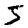
\includegraphics[width=.2\linewidth]{0.png}
  \caption{5}
  \label{fig:sub1}
\end{subfigure}%
\hspace{4mm}
\begin{subfigure}{.25\textwidth}
  \centering
  
\includegraphics[width=.2\linewidth]{1.png}
  \caption{0}
  \label{fig:sub2}
\end{subfigure}
\\
\begin{subfigure}{.25\textwidth}
  \centering
  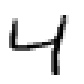
\includegraphics[width=.2\linewidth]{2.png}
  \caption{4}
  \label{fig:sub3}
\end{subfigure}
\begin{subfigure}{.25\textwidth}
  \centering
  
\includegraphics[width=.2\linewidth]{3.png}
  \caption{1}
  \label{fig:sub4}
\end{subfigure}
\caption{Sample Images}
\label{fig:test}
\end{figure}

Each image matrix is flattened into a one-dimensional vector. Then, a copy of the vector is converted from grayscale to black and white using Otsu’s Method. These vectors are then sent to the learning algorithms, which use a sample of 10,000 examples for training. After learning models are generating, they are tested against 10,000 similarly formatted test vectors.

\section*{Results}
\subsection*{Decision Trees}
Decision trees are graphs where each node represents a decision that asks a question about a certain feature. If the query is satisfied, the algorithm goes down one branch, otherwise it goes down another. This process repeats until a leaf node containing a final decision is encountered. In practice, a small decision tree that fits training data well is preferred over a larger tree. The smaller tree is superior because even if it has a slightly lower training accuracy, it is likely to generalize better, as the larger tree is probably learning random noise that helps classify the training data, but does not generalize to the testing data. This failure of the larger tree is often referred to as overfitting. To find a sufficiently complex tree, we experiment with a variety of restrictions on the maximum depth of the tree.

Unfortunately, finding the smallest accurate tree is a computationally complex. However, it is possible to find an approximately small tree using a greedy algorithm that selects nodes that maximize information gain. Information gain is a measure of the decrease in entropy - decisions that split many examples evenly between classes will have low information gain, whereas decisions that classify many examples into one specific class will have high information gain. If $pP$ represents the proportion of examples classified as positive, and $pN$ is the proportion of examples classified negative, then the entropy, $S$, is given by the following equation.
\[
S = -pP *\ log_2(pP) -pN * \log_2(pN)
\]
\begin{table}[ht!]
\centering
\caption{Decision Tree Results for Grayscale Images}
    \begin{tabular}{|l|l|}
    \hline
    Max Depth & Accuracy \\ \hline
    2      & 0.3363   \\ \hline
    4      & 0.611   \\ \hline
    8      & 0.796   \\ \hline
    16      & \textbf{0.8035}   \\ \hline
    32      & 0.8018   \\ \hline
    64      & 0.8018   \\ \hline
    128      & 0.8018   \\ \hline
    \end{tabular}
\end{table}

\begin{table}[ht!]
\centering
\caption{Decision Tree  Results for Black and White Images}
    \begin{tabular}{|l|l|}
    \hline
    Max Depth & Accuracy \\ \hline
    2      & 0.3324   \\ \hline
    4      & 0.5659   \\ \hline
    8      & 0.7692   \\ \hline
    16      & \textbf{0.8064}   \\ \hline
    32     & 0.8021   \\ \hline
	 64     & 0.8003   \\ \hline
   128    & 0.8062   \\ \hline
    \end{tabular}
\end{table}

\begin{figure}[h]
\centering
\begin{subfigure}{.45\textwidth}
  \centering
  \includegraphics[width=1\linewidth]{GrayscaleDecisionTrees.jpg}
  \caption{Grayscale Decision Trees}
  \label{fig:sub1}
\end{subfigure}%
\hspace{2mm}
\begin{subfigure}{.45\textwidth}
  \centering
  \includegraphics[width=1\linewidth]{BlackandWhiteDecisionTrees.jpg}
  \caption{Black and White Decision Trees}
  \label{fig:sub2}
\end{subfigure}
\caption{Decision Tree Results}
\label{fig:test}
\end{figure}

Compared to a majority vote baseline, which has accuracy $0.1135$, all of our decision trees perform better at the $0.01$ signifiance level according to a one tailed $t$-test. There is no significant difference between the best grayscale decision tree and the best black and white decision tree. This suggests that the thresholds calculated during each decision on the grayscale tree are roughly as good at classifying the data as Otsu's method. Interestingly, no significant overfitting occurs. While the accuracy of the grayscale tree does decrease after a depth of $16$, it is not by a significant amount.

\subsection*{Random Forests}
A variant of typical decision trees is to create a “forest” consisting of many randomly generated decision trees. Although each tree individually is more naive than the information gain decision trees, a collective vote from many trees is often more accurate and less prone to overfitting. We experimented with varying the maximum depth for each tree along with the number of trees in the forest.
\begin{table}[H]
\centering
\caption{Random Forest Results for Grayscale Images}
    \begin{tabular}{|l|l|l|}
    \hline
    Estimators & Max Depth & Accuracy \\ \hline
    1          & 2         & 0.3155   \\ \hline
    1          & 4         & 0.4495   \\ \hline
    1          & 8         & 0.6766   \\ \hline
    1          & 16        & 0.7608   \\ \hline
    1          & 32        & 0.7594   \\ \hline
    10         & 2         & 0.5604   \\ \hline
    10         & 4         & 0.7039   \\ \hline
    10         & 8         & 0.8814   \\ \hline
    10         & 16        & 0.9222   \\ \hline
    10         & 32        & 0.9241   \\ \hline
    50         & 2         & 0.5955   \\ \hline
    50         & 4         & 0.7557   \\ \hline
    50         & 8         & 0.9096   \\ \hline
    50         & 16        & 0.9501   \\ \hline
    50         & 32        & 0.9492   \\ \hline
    100        & 2         & 0.631    \\ \hline
    100        & 4         & 0.7766   \\ \hline
    100        & 8         & 0.9168   \\ \hline
    100        & 16        & 0.9531   \\ \hline
    100        & 32        & \textbf{0.9534}   \\ \hline
    \end{tabular}
\end{table}

\begin{table}[H]
\centering
\caption{Random Forest Results for Black and White Images}
    \begin{tabular}{|l|l|l|}
    \hline
    Estimators & Max Depth & Accuracy \\ \hline
    1          & 2         & 0.3277   \\ \hline
    1          & 4         & 0.4528   \\ \hline
    1          & 8         & 0.6684   \\ \hline
    1          & 16        & 0.7623   \\ \hline
    1          & 32        & 0.7553   \\ \hline
    10         & 2         & 0.4917   \\ \hline
    10         & 4         & 0.7128   \\ \hline
    10         & 8         & 0.8791   \\ \hline
    10         & 16        & 0.9164   \\ \hline
    10         & 32        & 0.9205   \\ \hline
    50         & 2         & 0.5887   \\ \hline
    50         & 4         & 0.7423   \\ \hline
    50         & 8         & 0.9027   \\ \hline
    50         & 16        & 0.9473   \\ \hline
    50         & 32        & 0.9467   \\ \hline
    100        & 2         & 0.5525    \\ \hline
    100        & 4         & 0.7504   \\ \hline
    100        & 8         & 0.9117   \\ \hline
    100        & 16        & 0.9504   \\ \hline
    100        & 32        & \textbf{0.9505}   \\ \hline
    \end{tabular}
\end{table}

\begin{figure}[h]
\centering
\begin{subfigure}{.45\textwidth}
  \centering
  \includegraphics[width=1\linewidth]{GrayscaleRandomForestsMaxDepth32.jpg}
  \caption{Grayscale Random Forests}
  \label{fig:sub1}
\end{subfigure}%
\hspace{2mm}
\begin{subfigure}{.45\textwidth}
  \centering
  \includegraphics[width=1\linewidth]{BlackandWhiteRandomForestsMaxDepth32.jpg}
  \caption{Black and White Random Forests}
  \label{fig:sub2}
\end{subfigure}
\caption{Random Forest Results}
\label{fig:test}
\end{figure}

According to a one tailed $t$-test, there is no significant difference between the best grayscale random forest classifer and the best black and white random classifier. In general, increasing the number of estimators improves the accuracy of the classifier. This makes sense, because having more classifiers means that it is less likely the majority of them will be wrong. Interestingly, the classifiers do not follow the same overfitting curve as regular decision trees. This could be because the trees are using a different information gain algorithm, or it could be because the random nature of the forest makes overfitting instances rare. In comparison to the majority vote baseline with an accuracy of $0.1135$, every random forest classifier performs significantly better.

During the random forest learning algorithm, each feature is given a value that represents how important that particular pixel is to determining the class of the number. The importances of each pixel can be graphed to produce a heat map showing which pixels reveal the most information about numbers.

\begin{figure}[H]
\centering
\begin{subfigure}{.4\textwidth}
  \centering
  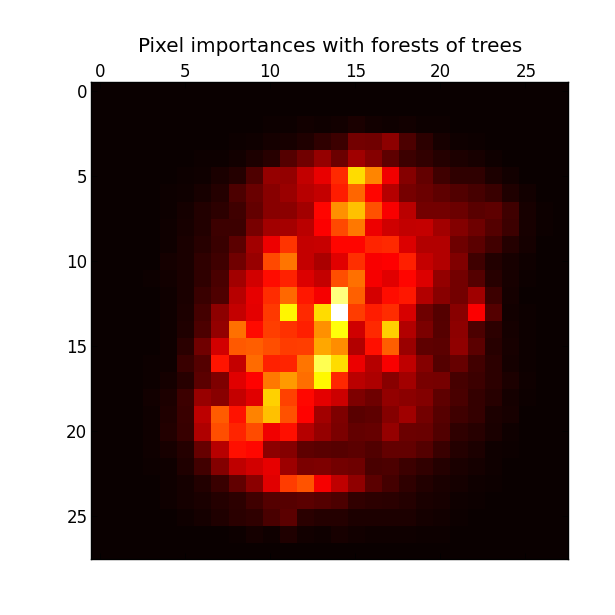
\includegraphics[width=1\linewidth]{gray_importances.png}
  \caption{Pixel Importances for Grayscale Images}
  \label{fig:sub1}
\end{subfigure}%
\hspace{4mm}
\begin{subfigure}{.4\textwidth}
  \centering
  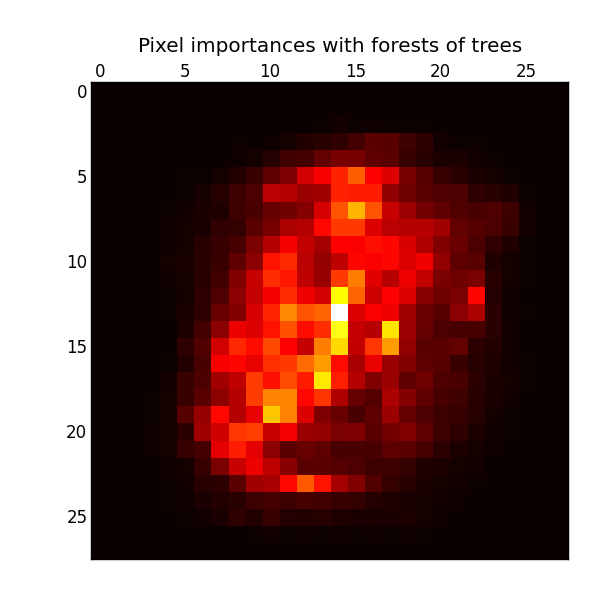
\includegraphics[width=1\linewidth]{bw_importances.png}
  \caption{Pixel Importances for Black and White Images}
  \label{fig:sub2}
\end{subfigure}
\end{figure}

Each picture looks almost exactly the same. This is additional evidence that black and white images perform similarly to grayscale images because the underlying decision algorithm is essentially the same. Unsurprisingly, each picture emphasizes the center areas where text is more likely to be present, with the greatest emphasis occuring in the middle pixel. 

\subsection*{Support Vector Machines}
Support Vector Machines attempt to find a hyperplane that separates data in a way that maximizes the distance between similar examples of different classifications, while also classifying training data correctly. While SVMs often achieve high accuracies, they have several serious weaknesses in the problem of handwriting classification. First, SVMs are inherently binary classifiers - for example, they determine whether a vector represents a 2 or does not represent a 2. In order to apply SVMs to multi-classification problems, it is necessary to run binary classification on an example against all ten possible digit classes, and then select the one in which the SVM has the most confidence. As the number of classes grows, this process becomes slow and less reliable. 

Another challenge SVMs face is that they typically linear classifiers, and not all data is best separated linearly. One approach to alleviating this limitation is to kernalize the data - that is, apply a function that maps inputs to higher dimension space. When the linear SVM is applied to the kernalized data and then downgraded to the original dimension, the result is data separated by a non-linear function. We experiment with polynomial kernels of various degrees. 

It should be noted that the parameter that measures the tradeoff between the size of the separating margin and the training accuracy (typically referred to as ‘c’) is not adjusted here, since no change in value made an appreciable increase in accuracy from the default.

\begin{table}[ht!]
\centering
\caption{SVM Results for Grayscale Images}
    \begin{tabular}{|l|l|}
    \hline
    Degree & Accuracy \\ \hline
    1      & 0.9123   \\ \hline
    2      & \textbf{0.9617}   \\ \hline
    3      & 0.9573   \\ \hline
    4      & 0.9464   \\ \hline
    5      & 0.9295   \\ \hline
    \end{tabular}
\end{table}

\begin{table}[ht!]
\centering
\caption{SVM Results for Black and White Images}
    \begin{tabular}{|l|l|}
    \hline
    Degree & Accuracy \\ \hline
    1      & \textbf{0.9098}   \\ \hline
    2      & 0.8427   \\ \hline
    3      & 0.1946   \\ \hline
    4      & 0.1135   \\ \hline
    5      & 0.1135   \\ \hline
    \end{tabular}
\end{table}

\begin{figure}[h]
\centering
\begin{subfigure}{.45\textwidth}
  \centering
  \includegraphics[width=1\linewidth]{GrayscaleSVMs.jpg}
  \caption{Grayscale SVMs}
  \label{fig:sub1}
\end{subfigure}%
\hspace{2mm}
\begin{subfigure}{.45\textwidth}
  \centering
  \includegraphics[width=1\linewidth]{BlackandWhiteSVMs.jpg}
  \caption{Black and White SVMs}
  \label{fig:sub2}
\end{subfigure}
\caption{SVM Results}
\label{fig:test}
\end{figure}

Compared to a majority vote baseline, which has accuracy $0.1135$, all of the SVMs perform better at the $0.01$ signifiance level according to a one tailed $t$-test. In summary, the best SVM model for grayscale performed better than the best SVM model for black and white at the $0.05$ signifcance level. One possible explanation that grayscale performed better in SVMs is that the SVM learning algorithm weights each feature as it trains. This creates a more native thresholding algorithm than Otsu's method. Another interesting observation is that the black and white SVMs performed very poorly with higher degree kernels. This suggests that after converting an image to black and white, the data becomes more linear than when it was in full grayscale.

\section*{Analysis}
\subsection*{Selection of Misclassifications}
To potentially improve our algorithm, it is worth analyzing misclassified images to detect any recurring problems. Some random samples of misclassified images are shown below.

\begin{figure}[h]
\centering
\begin{subfigure}{.25\textwidth}
  \centering
  
\includegraphics[width=.2\linewidth]{mistake[3]_5.png}
  \caption{Predicted 3, Actual 5}
  \label{fig:sub1}
\end{subfigure}%
\hspace{4mm}
\begin{subfigure}{.25\textwidth}
  \centering
  
\includegraphics[width=.2\linewidth]{mistake[7]_2.png}
  \caption{Predicted 7, Actual 2}
  \label{fig:sub2}
\end{subfigure}
\\
\begin{subfigure}{.25\textwidth}
  \centering
  
\includegraphics[width=.2\linewidth]{mistake[4]_9.png}
  \caption{Predicted 4, Actual 9}
  \label{fig:sub3}
\end{subfigure}
\begin{subfigure}{.25\textwidth}
  \centering
  
\includegraphics[width=.2\linewidth]{mistake[2]_4.png}
  \caption{Predicted 2, Actual 4}
  \label{fig:sub4}
\end{subfigure}
\caption{Sample Misclassifications}
\label{fig:test}
\end{figure}

In all four of the examples above, the numbers were written in an unorthodox or unclear way. For example, the first example looks like part of a 3 that was cut off, and the second example is a poorly drawn 2 that does look similar to a 7. The fact that the recognizer seems to misclassify mostly poorly drawn images is a good sign that its accuracy for decent handwriting is even higher than reported.

\subsection*{Confusion Matrix}
Another useful metric is to analyze which digits the recognizer is consistently confusing. This is shown visually with a confusion matrix. Each column of the matrix represents the predicted instances, and each row represents the true label. Therefore, the cell (0,1) shows the number of times the algorithm predicted 0 when the true label was 1. In the matrix below, the count of each error is multiplied by 15 in order to make errors more visually apparent. The classifier with the highest accuracy (SVMs of degree 2 with grayscale images) is used.

\begin{figure}[h]
\centering
  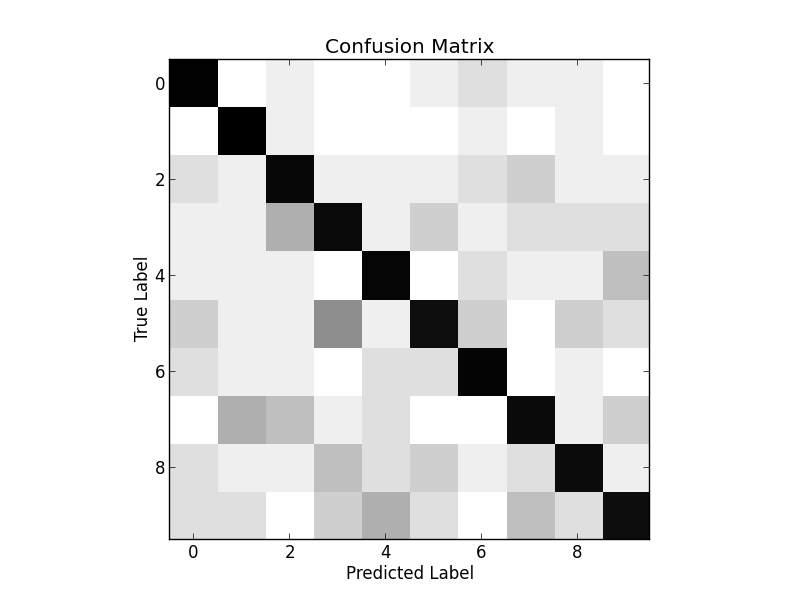
\includegraphics[width=.9\linewidth]{confusion.png}
  \caption{Confusion Matrix}
  \label{fig:conf}
\end{figure}

As expected, the diagonal representing correct guesses is most heavily populated. Some common points of confusion are to predict 3 when the label is actually 5, predicting 2 when the label is 3, and predicting 7 when the label is 9. 


\subsection*{Reducing Training Size}
One drawback of machine learning algorithms is that they require a large amount of training data to correctly classify characters. If the program is to generalize to all alphanumeric characters, rather than just digits, it would require even more training data. This data is often difficult to acquire and label, and takes up a large amount of space. Therefore, it is useful to see the tradeoff between the number of examples and the accuracy of the classifier. This relationship is shown below using the best classifiers for grayscale (SVMs of degree 2) and black and white images (random forests with 100 estimators of depth 32).
\begin{table}[H]
\centering
\caption{Grayscale Accuracy vs. Training Size}
    \begin{tabular}{|l|l|}
    \hline
    Training Size & Accuracy \\ \hline
    100      & 0.6549   \\ \hline
    500      & 0.8623   \\ \hline
    1000      & 0.9054   \\ \hline
    2000      & 0.9242   \\ \hline
    3000      & 0.9391   \\ \hline
    4000      & 0.9465   \\ \hline
    5000      & 0.9496   \\ \hline
    6000      & 0.9527   \\ \hline
    7000      & 0.9545   \\ \hline
    8000      & 0.9588   \\ \hline
    9000      & 0.9597   \\ \hline
    10000      & 0.9617   \\ \hline
    \end{tabular}
\end{table}

\begin{table}[H]
\centering
\caption{Black and White Accuracy vs. Training Size}
    \begin{tabular}{|l|l|}
    \hline
    Training Size & Accuracy \\ \hline
    100      & 0.6674   \\ \hline
    500      & 0.8336   \\ \hline
    1000      & 0.8901   \\ \hline
    2000      & 0.9157   \\ \hline
    3000      & 0.9301   \\ \hline
    4000      & 0.9375   \\ \hline
    5000      & 0.9415   \\ \hline
    6000      & 0.9433   \\ \hline
    7000      & 0.9484   \\ \hline
    8000      & 0.949   \\ \hline
    9000      & 0.9517   \\ \hline
    10000      & 0.9516   \\ \hline
    \end{tabular}
\end{table}

\begin{figure}[H]
\centering
\begin{subfigure}{.45\textwidth}
  \centering
  \includegraphics[width=1\linewidth]{GrayscaleSVMsExamples.jpg}
  \caption{Grayscale SVMs with Reduced Training Examples}
  \label{fig:sub1}
\end{subfigure}%
\hspace{2mm}
\begin{subfigure}{.45\textwidth}
  \centering
  \includegraphics[width=1\linewidth]{BlackandWhiteRandomForestsExamples.jpg}
  \caption{Black and White Random Forests with Reduced Training Examples}
  \label{fig:sub2}
\end{subfigure}
\caption{Reduced Training Examples}
\label{fig:test}
\end{figure}

Even with as few as 100 examples, both classifiers perform significantly better than the baseline accuracy. After about 1000 examples, the increase in training examples makes fairly little difference, and accuracy barely improves after 3000 examples. Interestingly, the learning curves are roughly the same, even though the underlying learning algorithms, SVMs and Random Forests, are different. This strongly suggests that the high number of training examples used in earlier experimentation was unnecessary, which makes more generalized handwriting recognition problems more tractable. 

\section*{Conclusion}
-Algorithms were very successful
-Overall no significant difference between BW and grayscale
-Generalize well to other digits, random forests better for that, no huge amounts of training necessary
-Future work to recognize whether something is a digit so that practical character reading can occur



\end{document}